\documentclass{beamer}

\usefonttheme{professionalfonts} % using non standard fonts for beamer
\usefonttheme{serif} % default family is serif

\usepackage{enumitem}
\setitemize{label=\usebeamerfont*{itemize item}%
  \usebeamercolor[fg]{itemize item}
  \usebeamertemplate{itemize item}}

\usepackage{hyperref}
%\usepackage{minted}
\usepackage{animate}
\usepackage{graphicx}
\def\Put(#1,#2)#3{\leavevmode\makebox(0,0){\put(#1,#2){#3}}}
\usepackage{colortbl}
\usepackage{tikz}
\usepackage{amssymb}
\usepackage{enumerate}
\usepackage{arydshln}
\usepackage{algorithm}
\usepackage{algpseudocode}
\usepackage{subcaption} %to have subfigures available

\usepackage[absolute,overlay]{textpos}

\colorlet{lightred}{red!25}
\colorlet{lightgreen}{green!25}
\beamertemplatenavigationsymbolsempty

\newcommand\blfootnote[1]{%
  \begingroup
  \renewcommand\thefootnote{}\footnote{#1}%
  \addtocounter{footnote}{-1}%
  \endgroup
}

\makeatletter

%% Textclass specific LaTeX commands.
\newcommand\makebeamertitle{\frame{\maketitle}}%
\AtBeginDocument{%
  \let\origtableofcontents=\tableofcontents
  \def\tableofcontents{\@ifnextchar[{\origtableofcontents}{\gobbletableofcontents}}
  \def\gobbletableofcontents#1{\origtableofcontents}
}
%% User specified LaTeX commands.
\usetheme{Malmoe}
\useoutertheme{infolines}
\addtobeamertemplate{headline}{}{\vskip2pt}
\setbeamercovered{transparent}

\title[PFlock report]{PFLOCK Report}
\author[AC]{Andres Calderon}
\institute[UCR]{University of California, Riverside}
\makeatother

%%%%%%%%%%%%%%%%%%%%%%%%%%%%%%%%%%%%%%
%% Main document
%%%%%%%%%%%%%%%%%%%%%%%%%%%%%%%%%%%%%%
\begin{document}
\makebeamertitle
\newif\iflattersubsect

\AtBeginSection[] {
    \begin{frame}<beamer>
    \frametitle{Outline} 
    \tableofcontents[currentsection]  
    \end{frame}
    \lattersubsectfalse
}

\AtBeginSubsection[] {
    \begin{frame}<beamer>
    \frametitle{Outline} 
    \tableofcontents[currentsubsection]  
    \end{frame}
}

\begin{frame}{On the spatial domain}{BFE overview...}
    \centering
    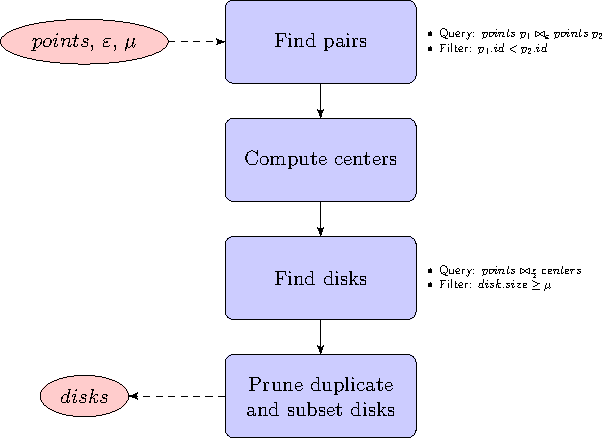
\includegraphics[width=0.7\textwidth]{figures/MF_flowchart}
\end{frame}

\begin{frame}{On the spatial domain}{BFE overview...}
    \centering
    \includegraphics[page=2,width=0.6\textwidth]{figures/grid}
\end{frame}

\begin{frame}{On the spatial domain}{BFE overview...}
    \centering
    \includegraphics[page=3,width=0.6\textwidth]{figures/grid}
\end{frame}

\begin{frame}{On the spatial domain}{BFE overview...}
    \centering
    \includegraphics[page=4,width=0.6\textwidth]{figures/grid}
\end{frame}

\begin{frame}{On the spatial domain}{BFE overview...}
    \centering
    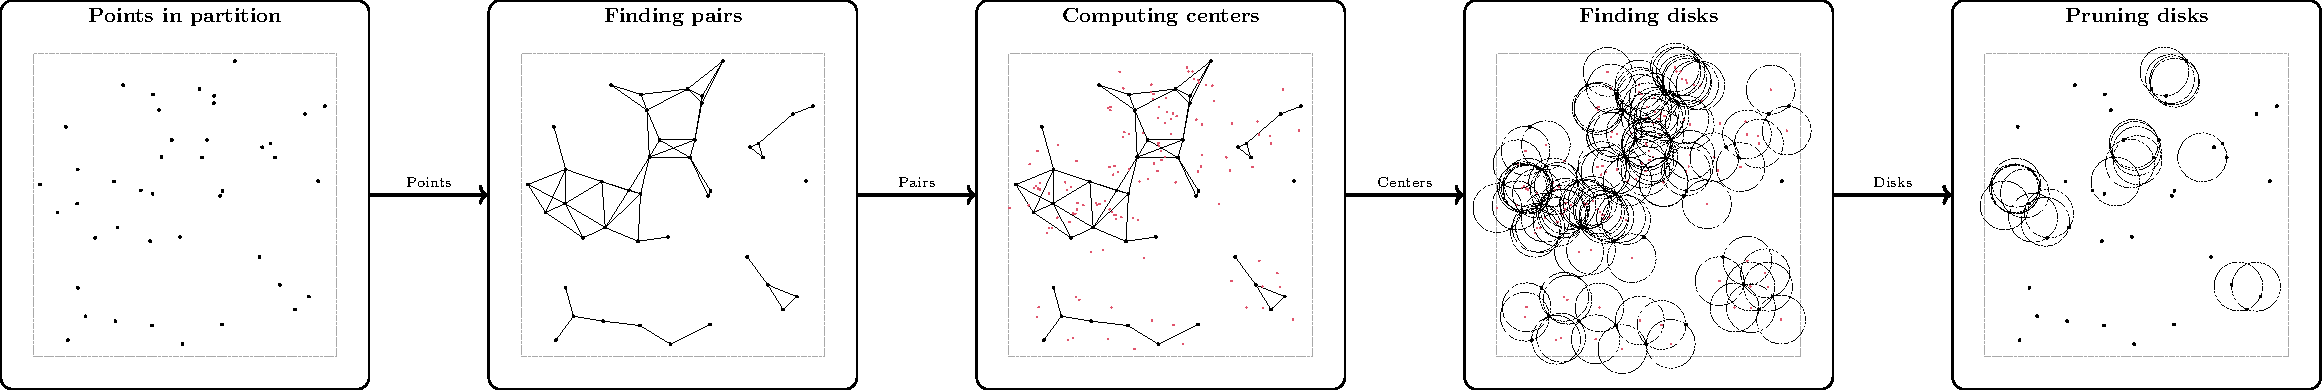
\includegraphics[width=\textwidth]{figures/MF_stages/flow}
\end{frame}

\begin{frame}{On the spatial domain}{Parallel overview...}
    \centering
    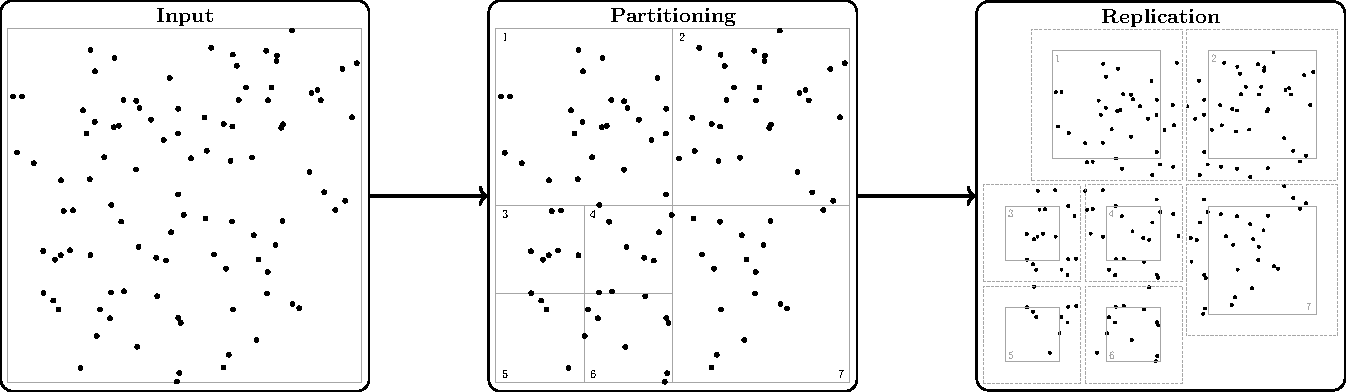
\includegraphics[width=\textwidth]{figures/MF_stages/P123}
\end{frame}

\begin{frame}{On the spatial domain}{Parallel overview...}
    \centering
    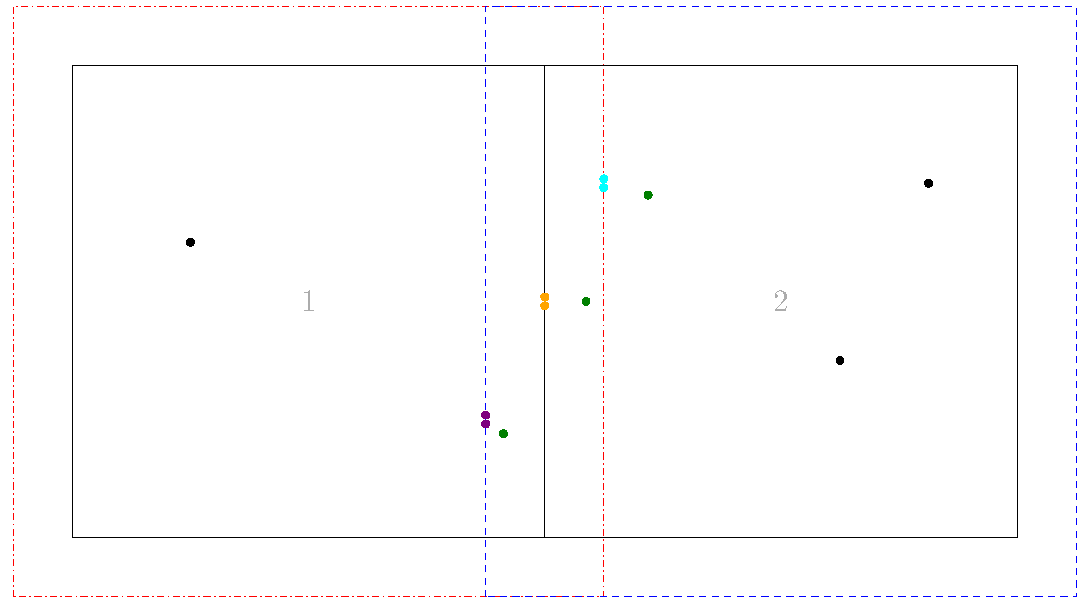
\includegraphics[page=1,width=\textwidth]{figures/merge}
\end{frame}

\begin{frame}{On the spatial domain}{Parallel overview...}
    \centering
    \includegraphics[page=2,width=\textwidth]{figures/merge}
\end{frame}

\begin{frame}{On the spatial domain}{Parallel overview...}
    \centering
    \includegraphics[page=3,width=\textwidth]{figures/merge}
\end{frame}

\begin{frame}{On the spatial domain}{Parallel overview...}
    \centering
    \includegraphics[page=4,width=\textwidth]{figures/merge}
\end{frame}

\begin{frame}{On the spatial domain}{Performance...}
    \centering
    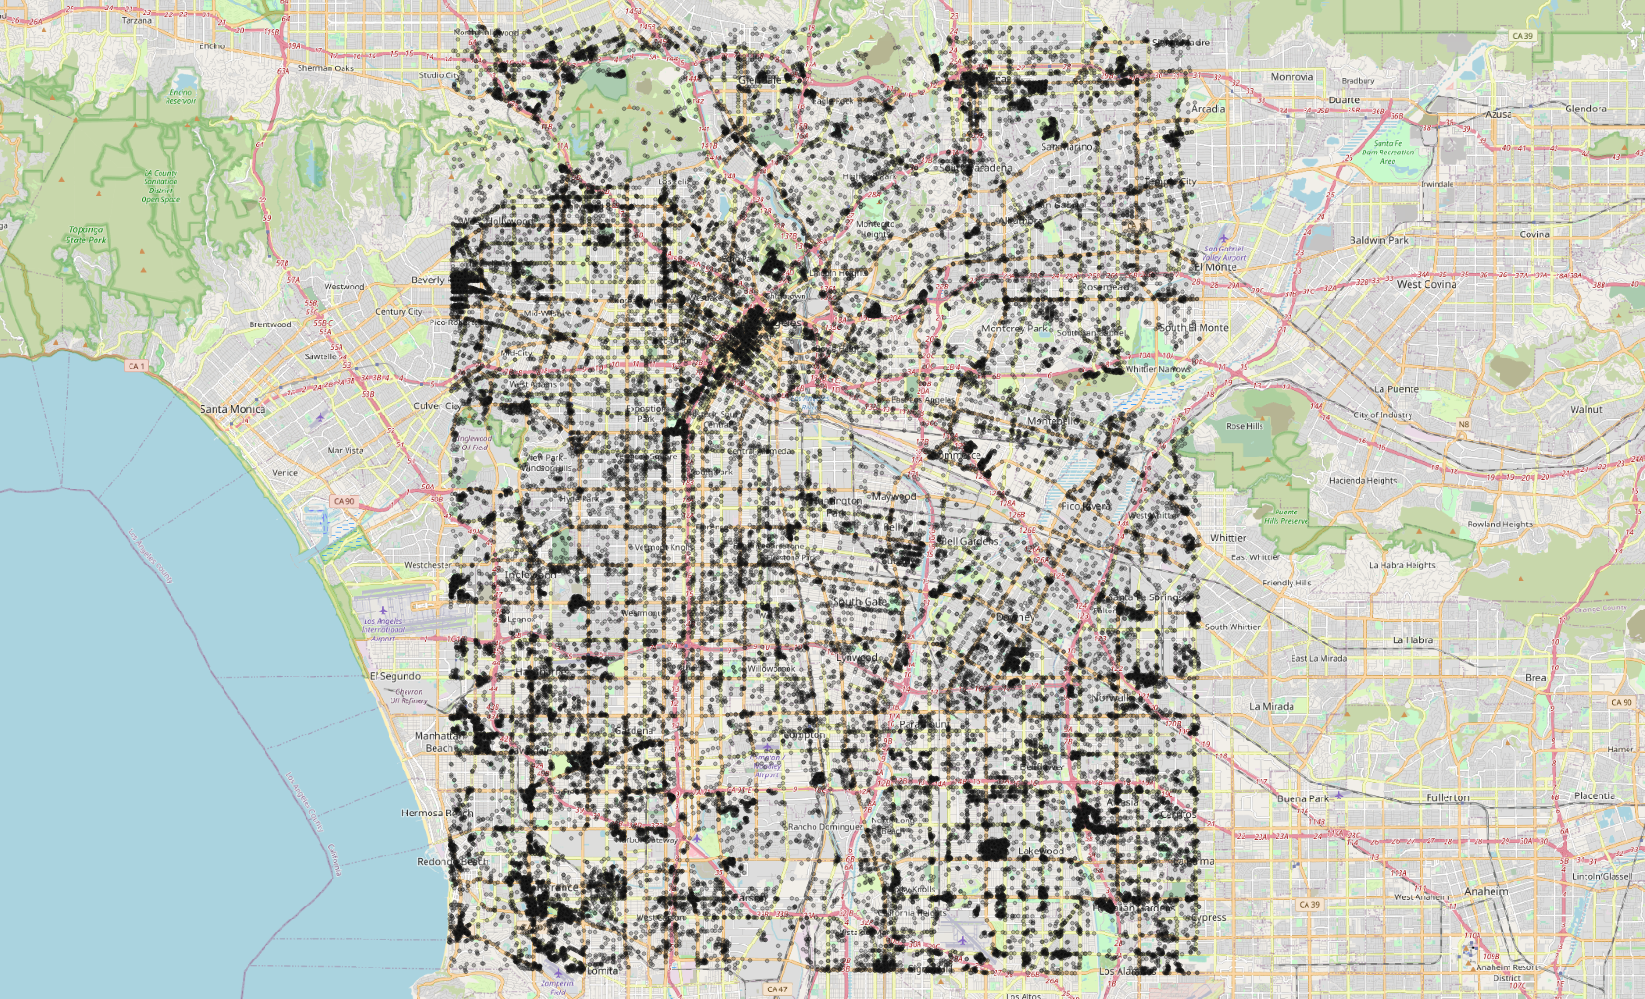
\includegraphics[width=0.9\textwidth]{/home/and/Research/Meetings/next/figures/LA_T320_N50K.png}
\end{frame}

\begin{frame}{On the spatial domain}{Performance...}
    \begin{figure}
        \centering
        \begin{subfigure}[t]{0.32\textwidth}
            \raisebox{-\height}{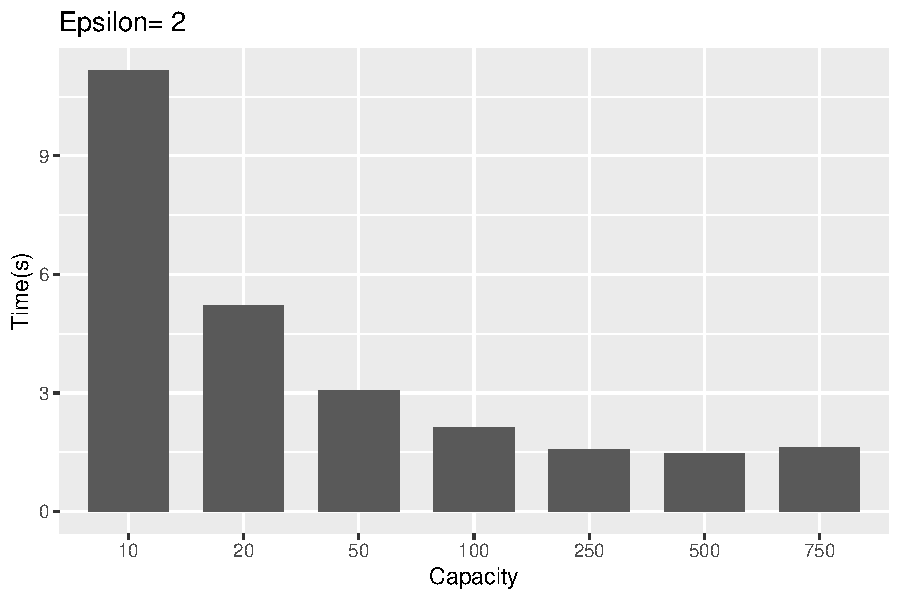
\includegraphics[width=\textwidth]{figures/R/MF/pflockE2_by_capacity}}
        \end{subfigure}
        \hfill
        \begin{subfigure}[t]{0.32\textwidth}
            \raisebox{-\height}{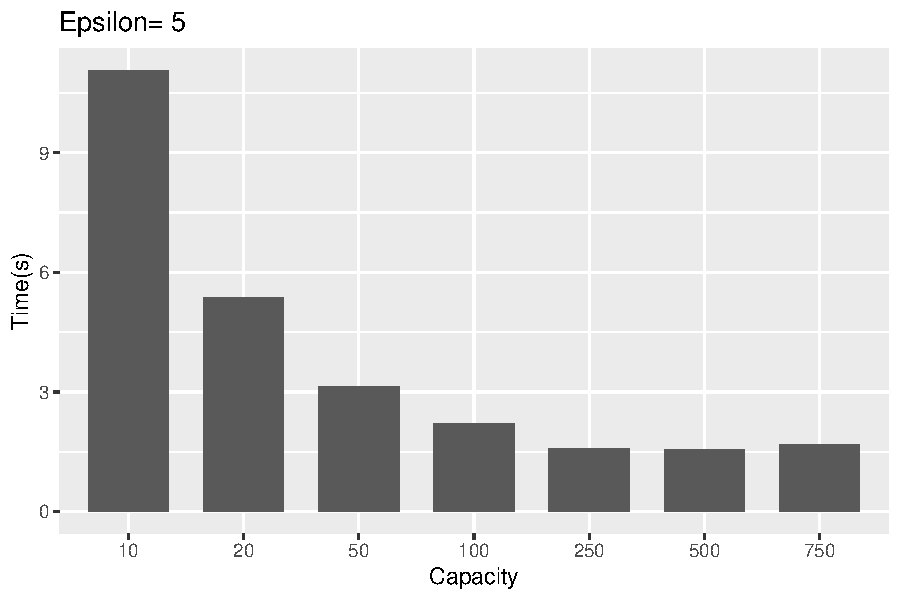
\includegraphics[width=\textwidth]{figures/R/MF/pflockE5_by_capacity}}
        \end{subfigure}
        \hfill
        \begin{subfigure}[t]{0.32\textwidth}
            \raisebox{-\height}{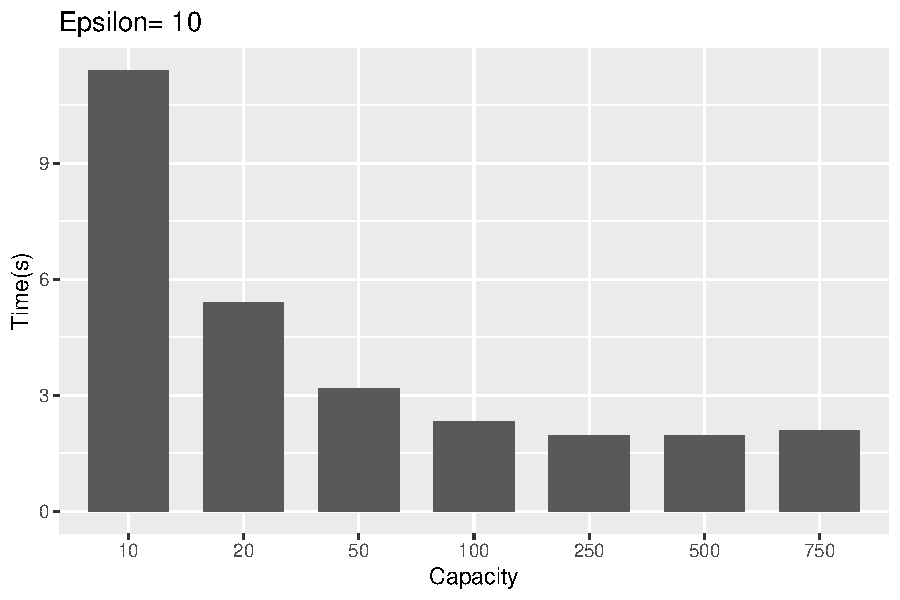
\includegraphics[width=\textwidth]{figures/R/MF/pflockE10_by_capacity}}
        \end{subfigure}
        %%%%%%%%%%%%%%%%%%%%%%%%%%%%%%%%%%%%second row
        \begin{subfigure}[t]{0.32\textwidth}
            \raisebox{-\height}{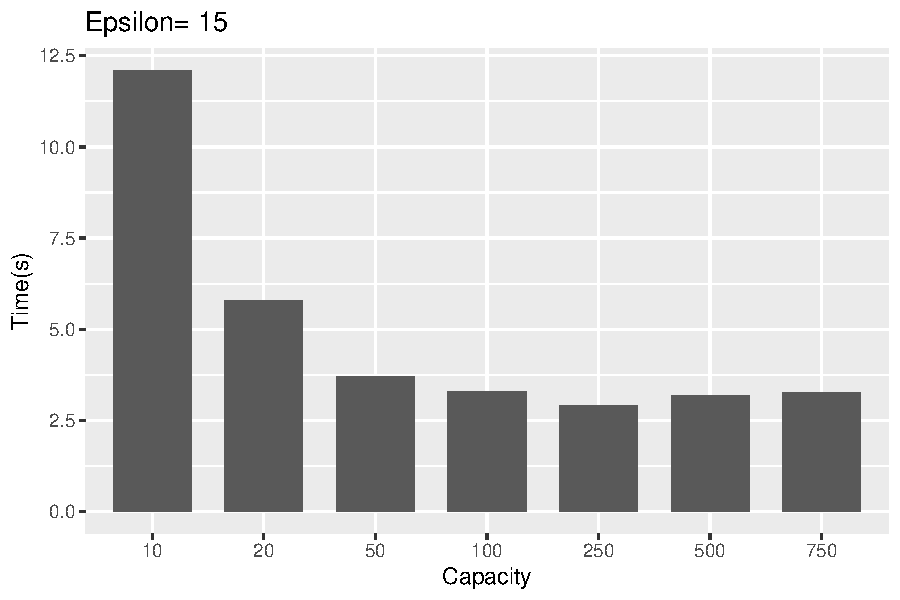
\includegraphics[width=\textwidth]{figures/R/MF/pflockE15_by_capacity}}
        \end{subfigure}
        %\hfill
        \begin{subfigure}[t]{0.32\textwidth}
            \raisebox{-\height}{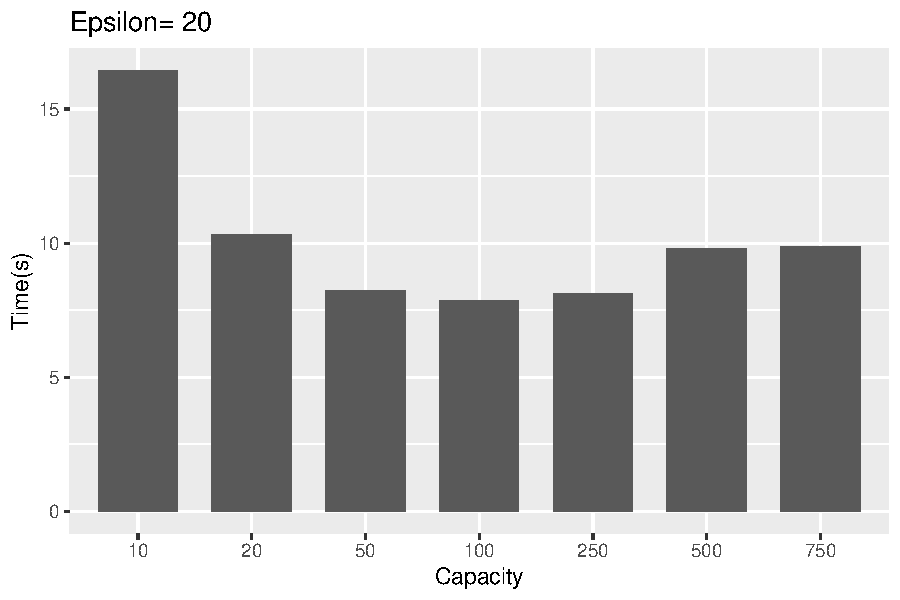
\includegraphics[width=\textwidth]{figures/R/MF/pflockE20_by_capacity}}
        \end{subfigure}
    \end{figure}
\end{frame}

\begin{frame}{On the spatial domain}{Performance...}
    \centering
    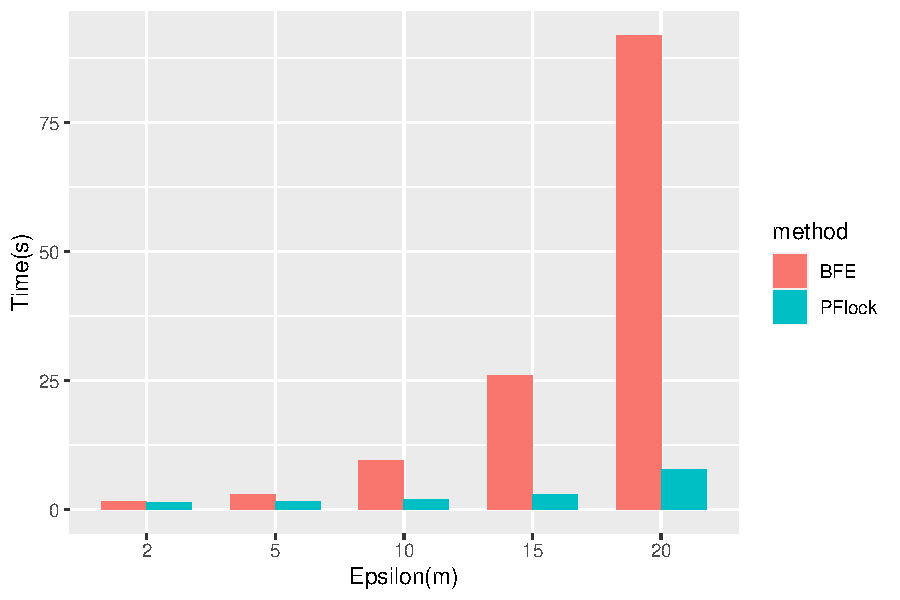
\includegraphics[width=0.9\textwidth]{figures/R/MF/PFlockVsBFE2.pdf}
\end{frame}

\begin{frame}{On the spatial domain}{Density issues...}
    \centering
    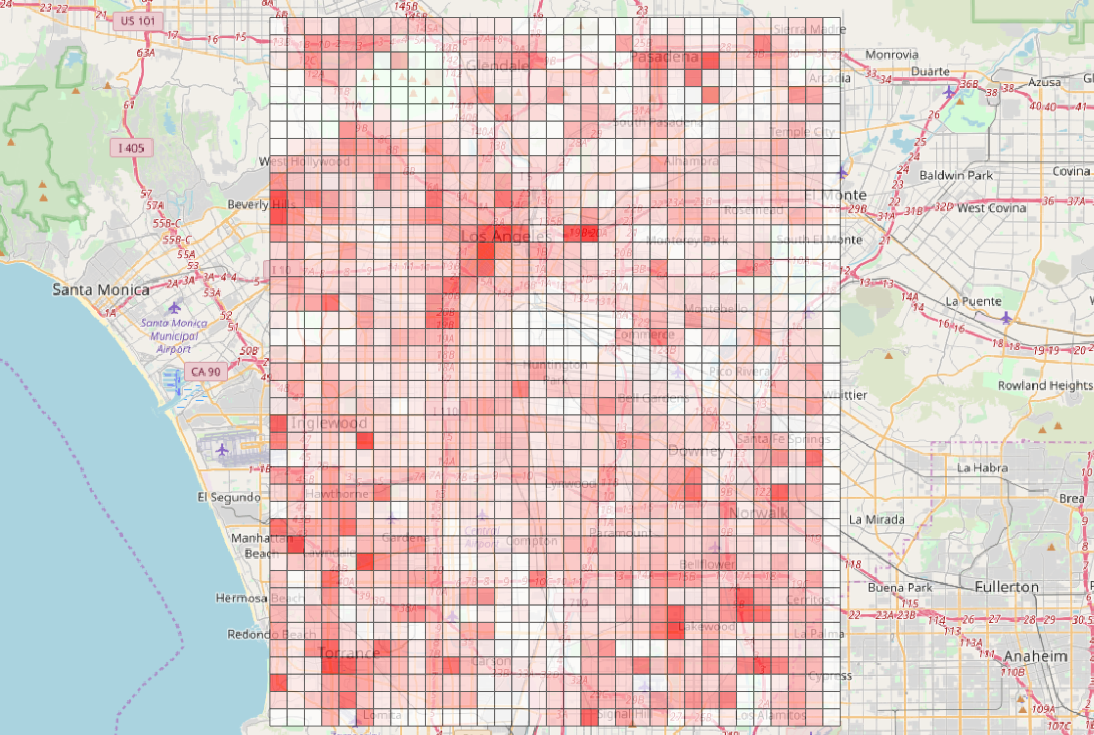
\includegraphics[width=0.8\textwidth]{figures/density.png}
\end{frame}

\begin{frame}{On the spatial domain}{Density issues...}
    \centering
    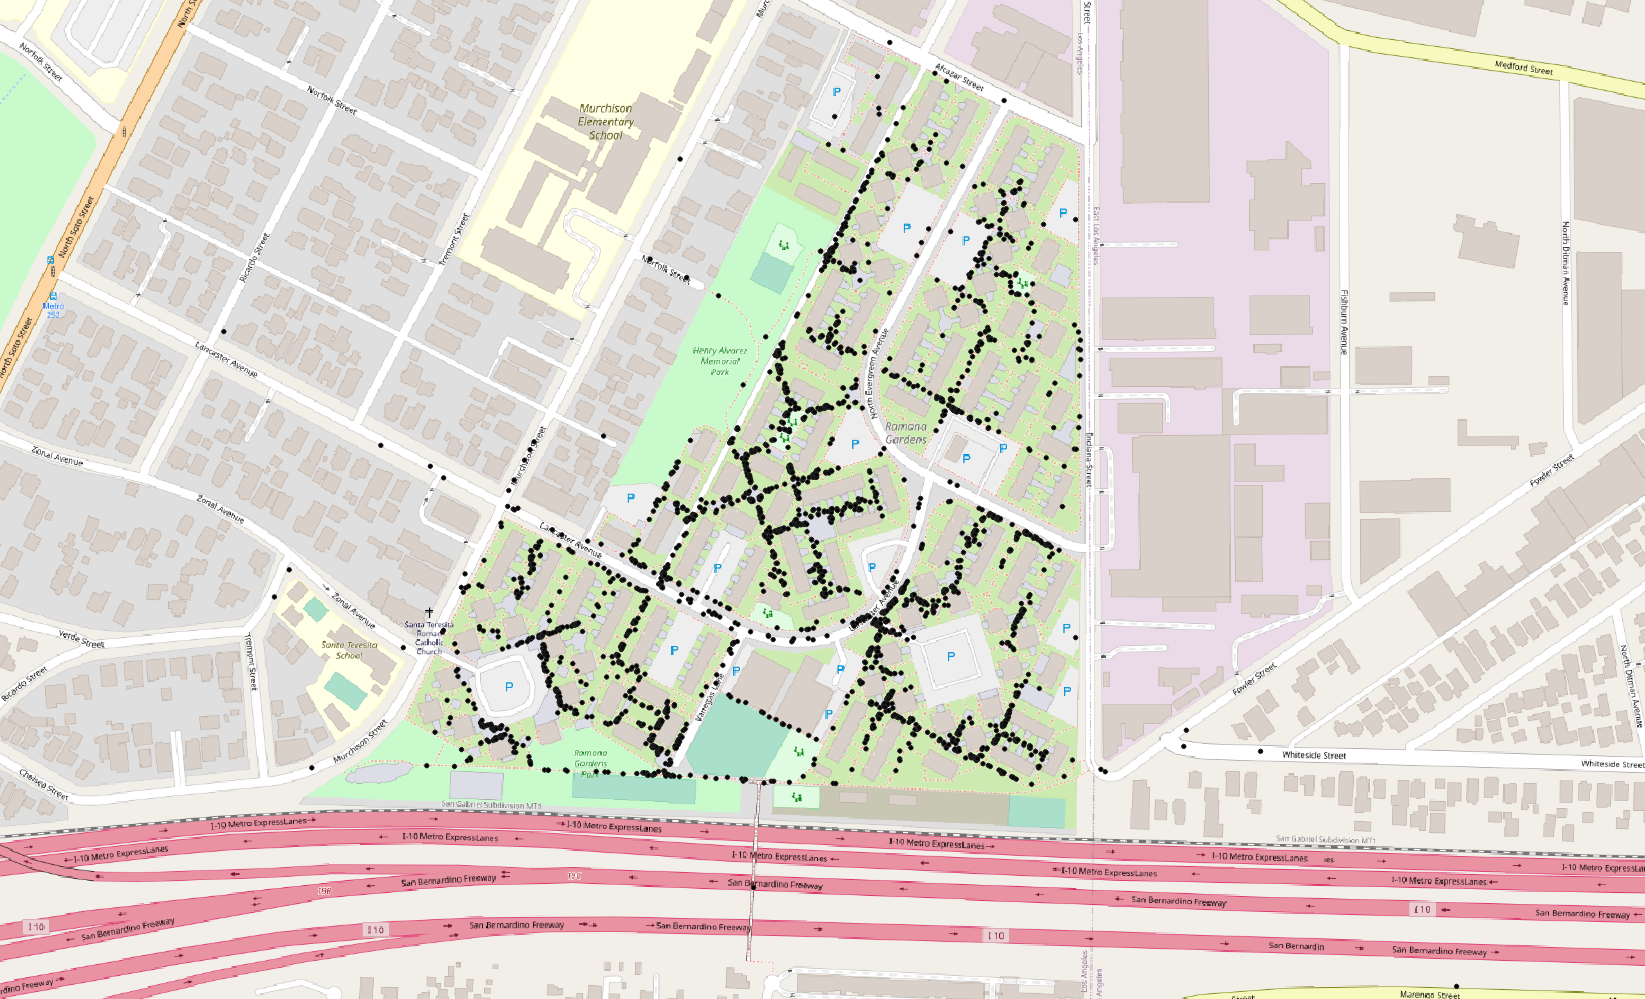
\includegraphics[width=0.9\textwidth]{figures/LA_T320_N50K_dense.png}
\end{frame}

\begin{frame}{On the spatial domain}{Cliques and MBCs approach...}
    \centering
    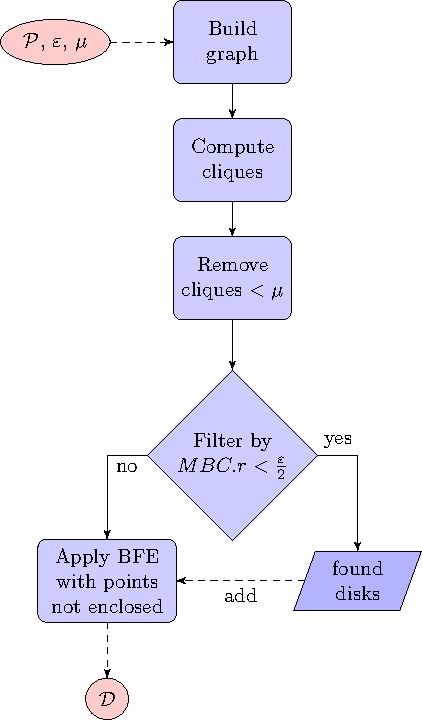
\includegraphics[width=0.5\textheight]{figures/CMBC_flowchart2.pdf}
\end{frame}

\begin{frame}{On the spatial domain}{Cliques and MBCs approach...}
    \begin{figure}
        \centering
        \begin{subfigure}[t]{0.49\textwidth}
            \raisebox{-\height}{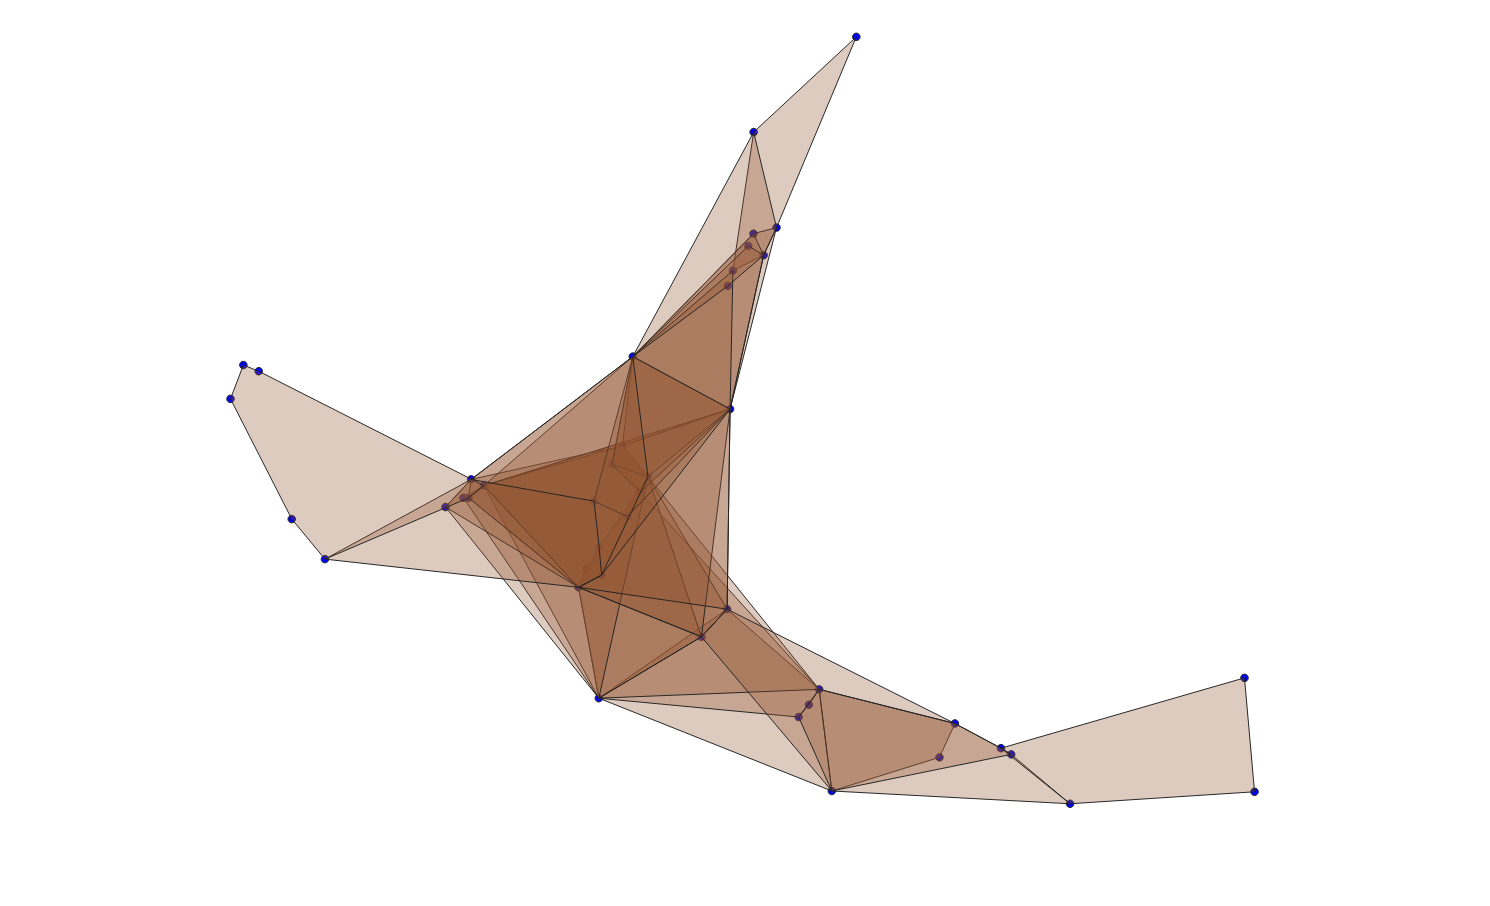
\includegraphics[width=\textwidth]{figures/CMBC1}}
            \subcaption{Finding cliques...}
        \end{subfigure}
        \hfill
        \begin{subfigure}[t]{0.49\textwidth}
            \raisebox{-\height}{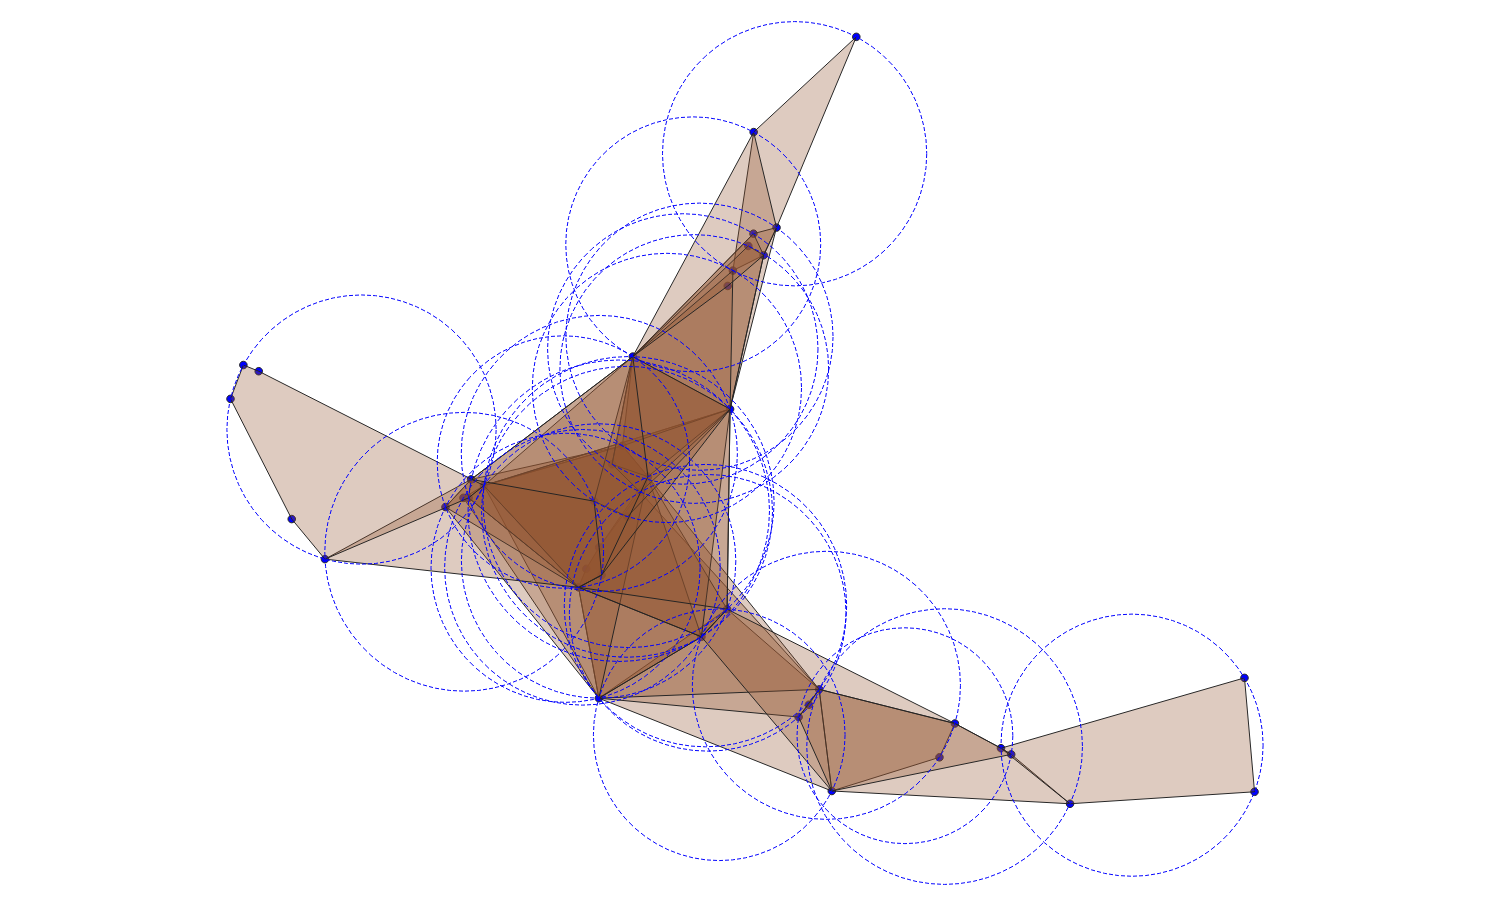
\includegraphics[width=\textwidth]{figures/CMBC2}}
            \subcaption{Filtering by MBC...}
        \end{subfigure}
    \end{figure}
\end{frame}

\begin{frame}{On the spatial domain}{CMBC performance (work in progress)...}
    \begin{figure}
        \centering
        \begin{subfigure}[t]{0.49\textwidth}
            \raisebox{-\height}{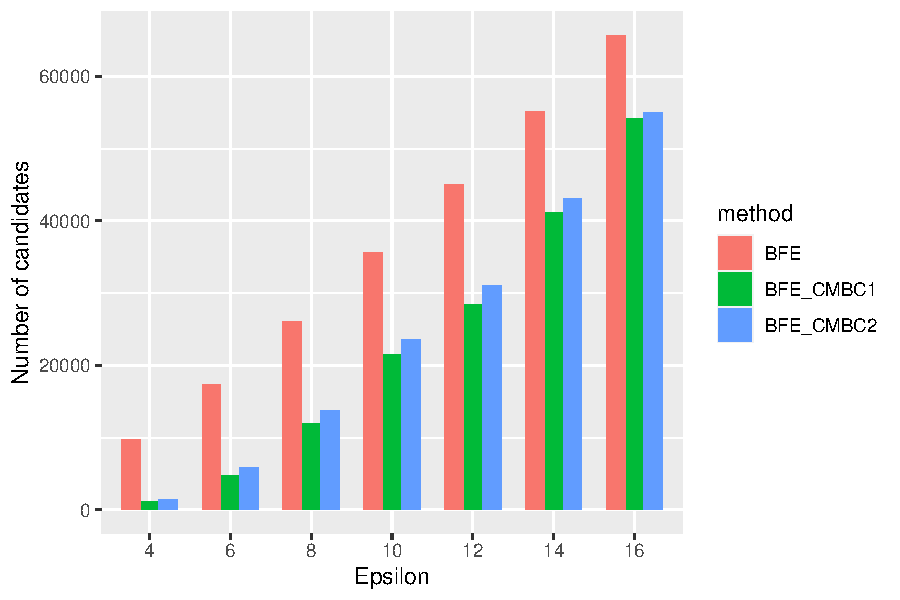
\includegraphics[width=\textwidth]{figures/R/CMBC/cmbc_by_candidates}}
            \subcaption*{It reduces the number of candidates...}
        \end{subfigure}
        \hfill
        \begin{subfigure}[t]{0.49\textwidth}
            \raisebox{-\height}{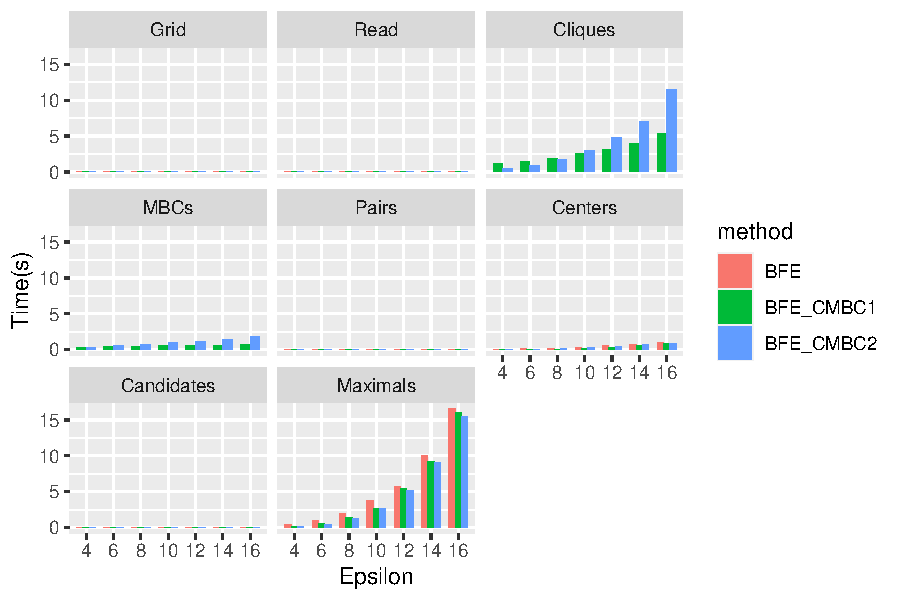
\includegraphics[width=\textwidth]{figures/R/CMBC/cmbc_by_time_stage}}
            \subcaption*{But it is quite costly...}
        \end{subfigure}
    \end{figure}
\end{frame}

\begin{frame}{On the time domain}{BFE overview...}
    \centering
    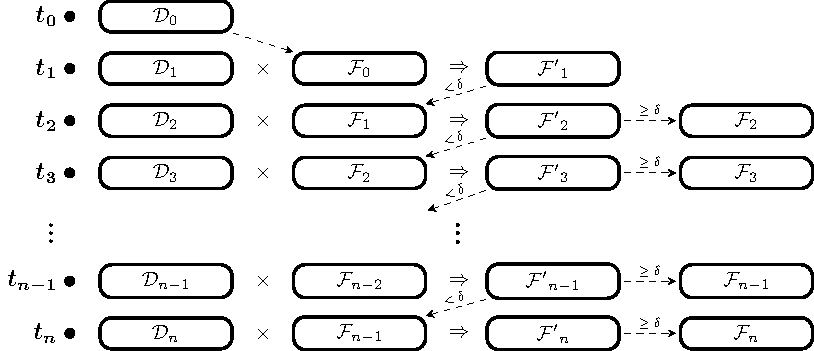
\includegraphics[height=0.55\textheight]{figures/FF_stages}
\end{frame}

\begin{frame}{On the time domain}{Proposal...}
    \centering
    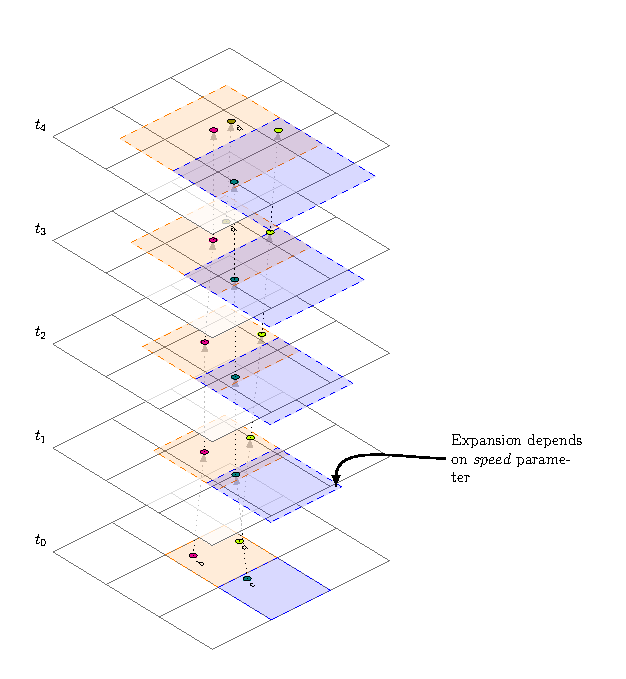
\includegraphics[height=0.85\textheight]{figures/TemporalPartitioning}
\end{frame}

\begin{frame}{What is next...}
    \begin{itemize}
     \item Double check CMBC approach.  If it prunes enough number of candidates it should gives us better times...
     \item Explore DBScan implementations\footnote{\url{https://link.springer.com/article/10.1007/s10115-016-1004-2}} to use instead of cliques...
     \item Give a try to distribute the neighborhood (stencil) during the PFlock parallelization...
     \item Time domain implementation...
    \end{itemize}

\end{frame}

\end{document}

